\documentclass[a4paper]{article} 
\usepackage{booktabs}
\usepackage{caption}
\usepackage{pythonhighlight}
\usepackage{pdfpages}
\usepackage{float}
\addtolength{\hoffset}{-2.25cm}
\addtolength{\textwidth}{4.5cm}
\addtolength{\voffset}{-3.25cm}
\addtolength{\textheight}{5cm}
\setlength{\parskip}{0pt}
\setlength{\parindent}{0in}

%----------------------------------------------------------------------------------------
%	PACKAGES AND OTHER DOCUMENT CONFIGURATIONS
%----------------------------------------------------------------------------------------

\usepackage{charter} % Use the Charter font
\usepackage[utf8]{inputenc} % Use UTF-8 encoding
\usepackage{microtype} % Slightly tweak font spacing for aesthetics
\usepackage[english,french]{babel} % Language hyphenation and typographical rules
\usepackage{amsthm, amsmath, amssymb} % Mathematical typesetting
\usepackage{float} % Improved interface for floating objects
\usepackage[final, colorlinks = true, 
            linkcolor = blue, 
            citecolor = lightblue]{hyperref} % For hyperlinks in the PDF
\usepackage{graphicx, multicol} % Enhanced support for graphics
\usepackage{xcolor} % Driver-independent color extensions
\usepackage{listings, style/lstlisting} % Environment for non-formatted code, !uses style file!
\usepackage{pseudocode} % Environment for specifying algorithms in a natural way
\usepackage[backend=biber,style=numeric,
            sorting=nyt]{biblatex} % Complete reimplementation of bibliographic facilities
\addbibresource{ecl.bib}
\usepackage{csquotes} % Context sensitive quotation facilities
\usepackage{fancyhdr} % Headers and footers
\pagestyle{fancy} % All pages have headers and footers
\fancyhead{}\renewcommand{\headrulewidth}{0pt} % Blank out the default header
\fancyfoot[L]{} % Custom footer text
\fancyfoot[C]{} % Custom footer text
\fancyfoot[R]{\thepage} % Custom footer text
\newcommand{\note}[1]{\marginpar{\scriptsize \textcolor{red}{#1}}} % Enables comments in red on margin
%----------------------------------------------------------------------------------------



%New colors defined below
\definecolor{codelightgreen}{rgb}{0,0.85,0}
\definecolor{codedarkgreen}{rgb}{0,0.4,0}
\definecolor{codelightred}{rgb}{0.95,0,0}
\definecolor{backcolour}{rgb}{0.95,0.95,0.95}
\definecolor{purple}{rgb}{0.8,0.2,0.8}

%Code listing style named "mystyle"
\lstdefinestyle{mystyle}{
  backgroundcolor=\color{backcolour},   
  commentstyle=\color{green},
  keywordstyle=\color{codelightgreen},
  numberstyle=\tiny\color{green},
  stringstyle=\color{codelightred},
  basicstyle=\footnotesize,
  breakatwhitespace=false,  
  breaklines=true,                 
  captionpos=b,                    
  keepspaces=true,                 
  numbers=left,                    
  numbersep=5pt,                  
  showspaces=false,                
  showstringspaces=false,
  showtabs=false,                  
  tabsize=2
}

%"mystyle" code listing set
\lstset{style=mystyle}

\theoremstyle{definition}
\theoremstyle{proposition}
\newtheorem{definition}{Definition}[section]
\newtheorem{proposition}{Proposition}[section]

\begin{document}

%-------------------------------
%	TITLE SECTION
%-------------------------------

\fancyhead[C]{}
\hrule \medskip % Upper rule
\begin{minipage}{0.295\textwidth} 
\raggedright
\footnotesize
Eric Benhamou, \hfill\\   
Marie Garin, \hfill\\   
Juliette Mansard, \hfill\\
Valentin Melot  \hfill\\
\end{minipage}
\begin{minipage}{0.4\textwidth} 
\centering 
\large 
Application to Journalism\\ 
\normalsize 
M2 MASH \\ 
Robin Ryder
\end{minipage}
\begin{minipage}{0.295\textwidth} 
\raggedleft
\today\hfill\\
\end{minipage}
\medskip\hrule 
\bigskip

%-------------------------------
%	CONTENTS
%-------------------------------

\section{Context}
The objective of this original and fruitful course was to set up an interaction between mathematics and journalists students in collaboration with the Institut Pratique du Journalisme. After being presented the problematic of Safety on roads, with a key focus on departmental road, we formed a group of 6 people (the 4 of us and 2 students from M2 IPJ: Cloe Ant and Antoine Cadaux) to analyze data from the \href{https://www.data.gouv.fr/fr/datasets/base-de-donnees-accidents-corporels-de-la-circulation/}{ONISIR data set}. We were asked to collaborate to find a journalistic problematic and illustrate the point of view with our statistical skills, in a traditional data journalism course. The overall idea was to study the data, find a problematic, propose and validate relevant models, perform mathematical analysis, choose an angle, develop some data visualizations. The journalist students were asked to write a report accessible to the general public in the form of a press article, while we were asked to write a more scientific one exposing our approach. We had 3 meeting together at the IPJ (Jan 16th, Feb 6th, and 27th). We summarize below our approach and findings and took the initiative to illustrate our point of view with relevant python code section and graphics. Full code is available at \href{https://github.com/ericbenhamou/MASH_IPJ_2018}{github}

\subsection{Subject}
We offer to study the mortality on road with a particular focus on departments (which was the keyword drawn randomly for our group). The theme is very up to date with the recent announcement of the prime minister Edouard Philippe about the speed reduction from 90 to 80 km/h on two way national and departmental roads (catr 2 and 3) in the database, which are equipped wit a central separator (circ other than 3).

The key findings are that these roads are actually the most dangerous according to the database of the ONISR (when looking at the criterion of danger: if you have an accident, proportion of serious or dead injuries). We try to give some hint about the impact of the measure (should it reduce mortality as much as promised). We also spent time to look at the statistics on these roads get an intuition of the causes and sources of accidents as well as possible solutions

\subsection{Description of the dataset}
The data set about personal injury of traffic in France is split into 4 different data sets listed by years on the website of the public administration and referred to as the  \href{https://www.data.gouv.fr/fr/datasets/base-de-donnees-accidents-corporels-de-la-circulation/}{ONISIR data set} given in csv format. In addition, a pdf file is given to describe the various fields and codes used in these data-sets. We investigated the data of year \textbf{2016}. Let us give briefly the characteristics:
\\
\\
The four sub databases are with self explained names
\begin{itemize}
\item vehicules
\item usagers
\item lieux
\item caracteristiques
\end{itemize}

They are easily loaded with pandas python library. These databases share in common the field \verb |Num_Acc| which refers to the code of the accident. An accident is reported by public forces (police or gendarmerie) if it has happened on a public lane and have involved at least one vehicle and at least one victim requiring care). We display below the characteristic of the various sub databases.
\begin{table}[H]
\centering
\caption{Database description}
\label{db_description}
\begin{tabular}{lllll}
dabase 		& number of rows & columns \\
usagers  		& 133,422 	& 12 \\
vehicules 		& 101,924	&  9 \\
lieux			&  59,432	& 18 \\
caracteristiques	&  59,432	& 16 
\end{tabular}
\end{table}

Because an accident involves on average about two or more vehicles and about two or more person, the database usagers and vehicles have roughly twice as much rows as he one corresponding to `lieux' and `caracteristiques' that have a unique row per accident. We put in the appendix section some descriptive statistics that are easily obtained by the pythonic command describe and easily converted into latex by the command on data frame \verb|to_latex| as shown by the small python snippet code below (full details in \href{https://github.com/ericbenhamou/MASH_IPJ_2018/tree/master/code}{github/MASH\_IPJ\_2018//code}). We have provided full details of the descriptive statistics in the appendix section \ref{Descriptive statistics}

\begin{lstlisting}[language=Python]
pd.options.display.float_format = '{:,.2f}'.format
for i, file in enumerate(files):
    print(dfs[i].drop('Num_Acc',axis=1).describe().to_latex())
    print('\captionof{table}{Descriptive stats for ', file, '}\n\\vspace{0.5cm}\n\n')
\end{lstlisting}
\bigskip

in 2016, the main points to note are:
\begin{itemize}
\item about 60,000 accidents have been declared
\item 3655 people died
\item 28,376 were reported as injured
\end{itemize}

\section{Exploratory phase}
Since we had to work on the specific subject of departmental roads, we started narrowing our data set. We plot first an histogram of the type of rods that are dangerous. 

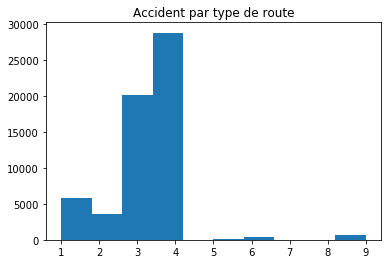
\includegraphics[width=8cm]{histo_roads_category.png}
\captionof{figure}{Accident per roads category: this histogram shows that accidents are mostly arriving on roads of category 3 and 4 which are `departementale' and `Voie Communale' roads, totaling about 85\% of accidents }
\vspace{0.5cm}

We can also look at a cross table to get a more detailed feeling of the re-partition of type of accidents per roads categories whcih is provided below

\begin{tabular}{lrrrrrrr}
\toprule
catr &    1 &    2 &    3 &    4 &    5 &    6 &    9 \\
grav &      &      &      &      &      &      &      \\
\midrule
1    & 0.45 & 0.39 & 0.36 & 0.44 & 0.37 & 0.44 & 0.41 \\
2    & 0.02 & 0.05 & 0.05 & 0.01 & 0.05 & 0.02 & 0.02 \\
3    & 0.13 & 0.22 & 0.31 & 0.16 & 0.30 & 0.25 & 0.22 \\
4    & 0.40 & 0.35 & 0.27 & 0.40 & 0.28 & 0.29 & 0.35 \\
\bottomrule
\end{tabular}
\captionof{table}{Repartition of accident per road categories: the label for the road cateories are the following:
'1': 'Autoroute', '2': 'Nationale', '3': 'Départementale', '4': 'Voie Communale', '5': 'Hors réseau public', '6': 'Parc de stationnement', '9': 'Autre'
while the ones for the type of accidents are 1: 'indemne', 2: 'tue', 3: 'blesse', 4: 'blesse leger'} \label{cross_tab1}

\vspace{0.5cm}
More visually, we can do a heat map as follows

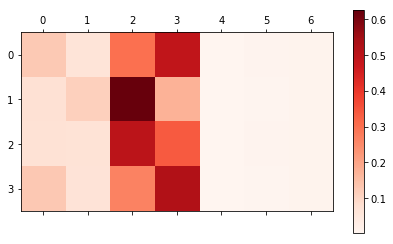
\includegraphics[width=8cm]{heatmap_roads_category_accident.png}\label{heatmap_roads_category_accident}
\captionof{figure}{heatmap per roads category and type: We can see visually that the most dangerous roads are by far the `Departementale' followed by `Communale' and the same applies for `wounded'. Because python starts at 0, the indexes correspond to the following: '0': 'Autoroute', '1': 'Nationale', '2': 'Départementale', '3': 'Voie Communale', '4': 'Hors réseau public', '5': 'Parc de stationnement', '6': 'Autre'
while the ones for the type of accidents are 0: 'indemne', 1: 'tue', 2: 'blesse', 3: 'blesse leger'}
\vspace{0.5cm}

in \ref{heatmap_roads_category_accident}, we see that  the two darkest columns are the one related to `'Départementale' and  'Voie Communale'. They represent 63\%, 17\% of death and 50\% and 34\% of wounded (see row 2 and 3 of table \ref{cross_tab1})

We also look at the presence or not of a `separateur central' as this makes the distinction between `national' with two separated lanes or not. We again use heat map and cross tab to build an intuition.
\begin{tabular}{lrrrrr}
\toprule
circ &  0.00 &  1.00 &  2.00 &  3.00 &  4.00 \\
grav &       &       &       &       &       \\
\midrule
1    &  0.07 &  0.19 &  0.56 &  0.17 &  0.01 \\
2    &  0.05 &  0.05 &  0.77 &  0.13 &  0.00 \\
3    &  0.07 &  0.12 &  0.70 &  0.11 &  0.01 \\
4    &  0.06 &  0.21 &  0.54 &  0.18 &  0.01 \\
\bottomrule
\end{tabular}


\captionof{table}{Cross table of gravity of the accident with the traffic type: the label for the road cateories are the following:
'1': 'Autoroute', '2': 'Nationale', '3': 'Départementale', '4': 'Voie Communale', '5': 'Hors réseau public', '6': 'Parc de stationnement', '9': 'Autre'
while the ones for the traffic types are '1': A sens unique, '2': – Bidirectionnelle, '3': A chaussées séparées, '4': Avec voies d’affectation variable }\label{cross_tab2}

with the corresponding heat map


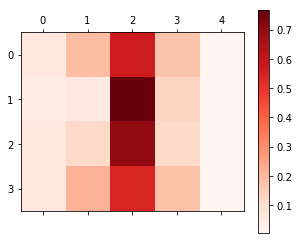
\includegraphics[width=8cm]{heatmap_roads_category_circ.png}\label{heatmap_roads_category_circ}
\captionof{figure}{heatmap per roads category and type: We can see visually that the most dangerous roads are by far the `Departementale' followed by `Communale' and the same applies for `wounded'. Because python starts at 0, the indexes are shifted by one compared to the table \ref{cross_tab2}}

Again this confirms our choice that `departementale', `communale' and `nationale' with no seperated lanes should be our key objectives. So we concentrate finally on bidirectional national roads and departmental without a `separateur central' (see our oral presentation available in \href{https://github.com/ericbenhamou/MASH_IPJ_2018/blob/master/presentation/presentation-2018-02-27.pdf}{presentation-2018-02-27.pdf} )

\newpage

In terms of coding, heatmap are easily done as follows:

\begin{lstlisting}[language=Python]
res2 = pd.crosstab(  tab['grav'].values, tab['trajet'].values, rownames =['gravite'],...)
plt.matshow( res2.values, cmap=cm.Reds, interpolation='none')
plt.colorbar()
plt.show()
\end{lstlisting}

%-----------------------------------------------------------------------------
% CHI SQUARE
%-----------------------------------------------------------------------------
\section{Chi square tests}
In this section we detail various Pearson correlation coefficient  tests done. Let us recall the assumptions of this test

\subsection{Assumtions}
The beauty of the R Correlation independence test is the simplicity of the assumptions.The two main important assumption to pay attention to are:

\subsubsection{Sample size assumption}
One can use the chi-square test to determine differences in proportions using a two-by-two contingency table. However it is crucial to note that chi-square tests yield only an approximated p-value. A correction factor has then to be applied. This only works when the data-sets are large enough. This is obviously our case. When sample sizes are small, a Fisher's exact test  should be more appropriate. A good rule of thumb is to have less than 20\% of the contingency cells with expected values less than 5 
In addition, the Fisher test is an exact test as opposed to the Chi square test. This means that the significance of the deviation from its null hypothesis can be calculated exactly, rather than relying on an approximation

\subsubsection{Independence assumption}
Secondly and more importantly, the chi-square test does not work on correlated data. For correlated data like when you are looking to test differences in proportions among matched pairs in a before/after scenario, an appropriate choice is the McNemar's test. In essence, this test is a chi-square goodness of fit test on the two discordant cells, with a null hypothesis stating that 50\% of the changes (agreements or disagreements) go in each direction. This test requires the same subjects to be included in the before and after measurements i.e. the pairs should be matched one-on-one.  

We can check that these two hypothesis are valid on our data-set. We now present the test framework.

\subsection{Test framework}
\begin{definition}
The Pearson correlation coefficient $\rho_{X,Y}$  also referred to as $r$, or $corr(X,Y)$  is defined for two time series $X$ and $Y$ as follows
\begin{equation}
\rho_{X,Y}= \frac{\sum ( X - \bar{X}) ( Y - \bar{Y} ) }  { \sqrt{  \left( \sum (X - \bar{X}) ^2 \right) \left(  \sum  (Y- \bar{Y}) ^2  \right) } }
\end{equation}
where $\bar(X) = \sum \frac{X}{N}$ , $\bar(Y) = \sum \frac{Y}{N}$. The formula above is easier to understand but is not the most efficient one to compute as it computes too similar terms multiple times. In practice, one uses the following faster formula

\begin{equation}
\rho_{X,Y} = \frac{\sum ( X Y - \bar{X} \bar{Y} ) }  { \sqrt{  \left( \sum (X^2 - \bar{X}^2 \right) \left(  \sum  (Y^2 - \bar{Y} ^2  \right) } }
\end{equation}

anoter interpretation of the formula is in terms of expectation as follows;
\[
\rho_{X,Y}=\frac{\operatorname{E}[(X-\mu_X)(Y-\mu_Y)]}{\sigma_X\sigma_Y} 
\]

where:
$\sigma_X $  is the standard deviation of $X$
$\mu_X$ is the mean of $X$
$\operatorname{E}$ is the expectation.

\end{definition}

We have the following properties
\begin{proposition}
The absolute values of the sample Pearson correlation coefficients is less than or equal to 1. Correlations equal to 1 or -1 correspond to data points lying exactly on a line (in the case of the sample correlation), or to a bi-variate distribution entirely supported on a line. The Pearson correlation coefficient is symmetric: 
\[ 
\rho_{X,Y}= \rho_{Y,X}
\]
\end{proposition}

\begin{proposition}
A key mathematical property of the Pearson correlation coefficient is that it is invariant under separate changes in location and scale in the two variables. That is, we may transform $X$ to $ a + bX$ and transform $Y$ to $c + dY$, where $a, b, c,$ and $d$ are constants with $b, d > 0$, without changing the correlation coefficient. Note that more general linear transformations do change the correlation
\end{proposition}

A powerful property is that this statistic can be used to test independence of two variables.\newline


\textbf{Test hypothesis} \newline
We want to test \textbf{H0:} There is no relationship between the variables $X$ and $Y$ versus \textbf{H1:} There is a relationship between the variables $X$ and $Y$



\begin{proposition}
Using a permutation test, we can compute a p-value to reject or to fail to reject H0 as follows, called permutation test in the following two steps: 

\begin{enumerate}
\item  Using the original paired data $(x_i,y_i)$, randomly redefine the pairs to create a new data set $(x_i,y_{i'})$ where the index $i'$ are a permutation of the set ${1,...,n}$.  
The permutation $i'$  is selected randomly, with equal probabilities placed on all $n!$ possible permutations.  
This is equivalent to drawing the $i'$ randomly without replacement from the set ${1, ..., n}$.  
A closely related and equally justified bootstrapping approach is to separately draw the $i$ and the $i'$  ''with replacement'' from  set ${1, ..., n}$
\item Construct a correlation coefficient $\rho_{X,Y}$ from the randomized data.
\end{enumerate}

To perform the permutation test, repeat steps (1) and (2) a large number of times.  The p-value for the permutation test is the proportion of the $\rho_{x,y}$ values generated in step 2 that are larger than the Pearson correlation coefficient that was calculated from the original data.  Here "larger" can mean either that the value is larger in magnitude, or larger in signed value, depending on whether a two-sided or one-sided test is desired.
\end{proposition}

Chi square tests are easily done in Python thanks to the scipy library. This is written in two lines as follows
\begin{lstlisting}[language=Python]
import scipy.stats as scs
chisq_test = scs.pearsonr(tab['has_tpc'].values, tab['mort_ou_grave'].values)
correlation = chisq_test[0]
p_value = chisq_test[1]
print("La correlation est de {:.2f}.".format(correlation))
print("La p-value est de {:.2e}.".format(p_value))
\end{lstlisting}

It is worth mentioning that one has to merge table in order to address data cross tables. This is done easily with pandas as follows
\begin{lstlisting}[language=Python]
db_combined = dfs[0]
for i in range(3):
    db_combined = db_combined.merge(dfs[i+1], on='Num_Acc',how='left')
\end{lstlisting}


\subsection{Visual representation}
In order to graphically visualize a Chi square test, we develop an original method. We plot the contingency table as a mosaic matrix and draw on the cross the confidence intervals that confirm that the two variables are independent using a standard chi square test. This is quite original in terms of visualizing the chi square test as statisticians usually just refer to the p-value but they do not give a visual representation of the test. 

To our knowledge \textbf{this is new}. 
To illustrate this, let us look at the first test we did which was to validate or not that the presence of a `terre-plein' central saves lifes or not. We ran a Pearson correlation coefficient and retrieve the corresponding p-value for testing non-correlation.
The test is simply executed by the pythonic code  scs.pearsonr and provided a p-value of 8.85e-156 and a correlation of -11.4%

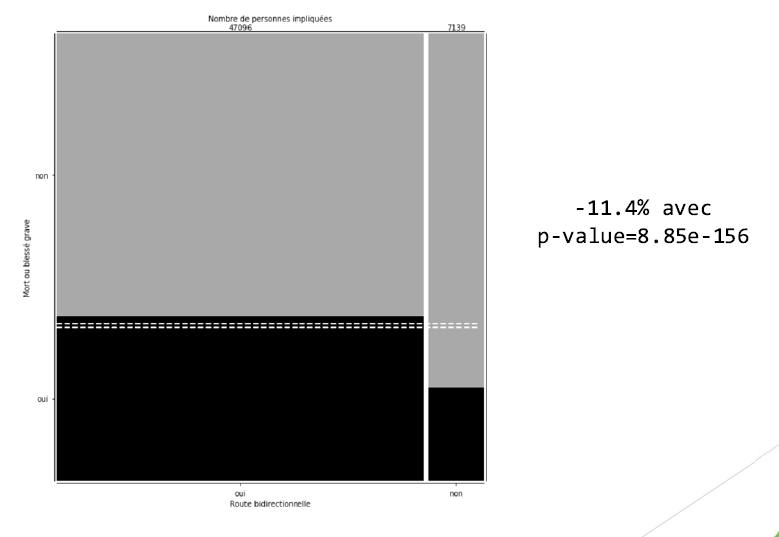
\includegraphics[width=8cm]{indep_1_test.png}\label{indep_1_test}
\captionof{figure}{original representation of the Pearson test of independence: We can see that the presence of a terre plein central is clearly not independent of the death or not within an accident as both the Yes and No categories are not within the dashed line band that indicate the range for independence}

We present in appendix a collection of independence test done using both the traditional test test and visual test \ref{Independence_testing}

The full code for the visualization that we do not reproduce here for obvious reason of readability (about 100 lines of code) is located in the python jupyter notebook \verb|code/DataVisualisation.ipynb| 
The key function is \verb|mosaic_plot| whose usage is trivial and given for instance by

\begin{lstlisting}[language=Python]
#Mosaic plot survivant vs. sexe
ct_grav_sex = pd.crosstab(accidents_int["grav_fatal"], accidents_int["sexe_cond"])
N = np.sum(ct_grav_sex.values)
phat = np.sum(ct_grav_sex.values[0,:]) / N
deltap = scs.norm.ppf(.975) * np.sqrt(phat * (1-phat) / N)
mosaic_plot(ct_grav_sex, {False: "darkgrey", True: "black"}, figsize=(10,10), pad_x=.01, pad_y=0,
            x_label="Sexe du conducteur", y_label="Mort ou gravement blesse",
            row_labels=["non", "oui"],
            col_labels=["homme", "femme"],
            top_label="Nombre de personnes impliquees",
            lines=[(phat+deltap, "w--", {"linewidth": 2}),
                   (phat-deltap, "w--", {"linewidth": 2})])
\end{lstlisting}






%-----------------------------------------------------------------------------
% lOGISTIC REGRESSION
%-----------------------------------------------------------------------------
\section{Logistic regression}
We also performed some logistic regression. The framework is given below

\subsection{Assumptions}
Logistic regression relies on a few assumption and much less than the ones of linear regression and general linear models. Let us explain this in more details
\subsubsection{Assumptions for logistic regression}

\begin{proposition}
We summarized below the key assumptions of logistic regression (LR)
\begin{enumerate}
\item LR requires the dependent variable to be binary or ordinal 
\item LR  requires the observations to be independent of each other.  In other words, the observations should not come from repeated measurements or matched data.
\item LR  requires there to be little or no multi col-linearity among the independent variables.  This means that the independent variables should not be too highly correlated with each other.
\item  LR  assumes linearity of independent variables and log odds.  Although this analysis does not require the dependent and independent variables to be related linearly, it requires that the independent variables are linearly related to the log odds.
\item LR requires a large sample size.  A rule of thumb is that you need at minimum of 10 cases with the least frequent outcome for each independent variable in your model. 
For example, if you have 5 independent variables and the expected probability of your least frequent outcome is 0.10, then you would need a minimum sample size of 500= (10*5 / .10).
\end{enumerate}
\end{proposition}

\subsubsection{Difference with linear regression}
\begin{proposition}
Logistic regression differs substantially from linear regression assumptions, summarized below
\begin{enumerate}
\item no need for a linear relationship between the dependent and independent variables.  
\item no assumption of normality of residual terms
\item no homoscedasticity 
\item no continuous variable for y
\end{enumerate}
\end{proposition}


\subsection{Framework}
Logistic regression is the appropriate regression analysis to conduct when the dependent variable is dichotomous (binary) or ordinal as opposed to continuous variables that requires regular linear regression and its extension. Logistic regression is predictive analysis, in the sense that it can be use to predict conclusion on new data. Logistic regression is mostly used to describe data and to explain the relationship between one dependent binary variable and one or more nominal, ordinal, interval or ratio-level independent variables. Let us present the framework.

Mathematically, logistic regression or logit model is a binomial regression and defined as follows
\begin{definition}
The logit probability is defined as
\[
\text{logit}(p)= \log\left( \frac{ \mathbf{P}(Y=1)} { \mathbf{P}(Y=0)} \right)
\] 
\end{definition}

The logistic regression is then obtained by regressing the logit variable over the explanatory variables as follows
\begin{proposition}
Logistic regression consists in regressing the logit variable over the constant and $X$ as follows
\[
\text{logit}(p)= a + B X + \epsilon
\]
where $\epsilon$ are the residuals, $a$ is the intercept term while $B$ is the matrix of weights. We can obviously write a more general form if we include in the variables $X$ the constant vector.
The coefficient terms $a$ and $B$ are estimated via maximum likelihood. Practically, software do not try to solve the problem but rather for an approximation of the solution using numerical solution thanks to Iteratively reweighed least squares (IRLS) using Newton's method (for more details, this was seen in Probabilistic Graphical Method and implemented in homework 1). In order to evaluate the quality of fit and prevent over-fitting, it is useful to visualize the confusion matrix.
\end{proposition}


\subsection{Illustration}
We run a test to do a logistic regression on bikers and `glissieres'. Since the coefficient for $X1$ is negative, it indicates that `glissieres' saves life but the coefficient for $X2$ and $X3$ e
\begin{verbatim}
Optimization terminated successfully.
         Current function value: 0.688725
         Iterations 5
                         Results: Logit
=================================================================
Model:              Logit            Pseudo R-squared: -0.047    
Dependent Variable: mort_ou_grave    AIC:              64878.3598
Date:               2018-03-09 08:57 BIC:              64904.6396
No. Observations:   47096            Log-Likelihood:   -32436.   
Df Model:           2                LL-Null:          -30990.   
Df Residuals:       47093            LLR p-value:      1.0000    
Converged:          1.0000           Scale:            1.0000    
No. Iterations:     5.0000                                       
--------------------------------------------------------------------
       Coef.     Std.Err.       z       P>|z|      [0.025     0.975]
--------------------------------------------------------------------
x1    -0.3685      0.0895    -4.1148    0.0000    -0.5440    -0.1930
x2     0.4503      0.0245    18.3757    0.0000     0.4023     0.4983
x3     1.4484      0.2580     5.6145    0.0000     0.9428     1.9540
=================================================================

\end{verbatim}


The corresponding python code for running a logistic regression is like for the Chi square test trivial and consists on a few lines as follows

\begin{lstlisting}[language=Python]
import statsmodels.api as sm
import scipy 
import numpy as np

y=tab['mort_ou_grave']
tab['moto'] = np.logical_and( tab['catv'] <= 34, tab['catv'] >= 30 )
X=np.column_stack( (tab['glissiere'].values, tab['moto'].values,  tab['moto'].values * tab['glissiere'].values) )
logit_model = sm.Logit(y,X)
result = logit_model.fit()
print(result.summary2())
\end{lstlisting}

%-----------------------------------------------------------------------------
% KEY FINDINGS
%-----------------------------------------------------------------------------
\section{Key findings}
\begin{itemize}
\item departmentale, communale and national roads without `terre plein centrale' are the most dangerous ones.
\item the presence of a terre plein central saves life
\item the type of roads matters. Departementale are the most dangerous.
\item we can draw the profile of the typical driver that kills on roads. The driver is a young or senior (more than 65 year old). It is mostly a male
\item we can also infer the type of situations that are dangerous: tree on the sides 
\item last but not least, `glissiere' saves life but are dangerous for bikers.
\end{itemize}

\section{Conclusion}
This three session about data journalism have been exciting. Through the constant interaction with journalist students, we have been able to better understand the issue of communication between the scientists and journalists. This becomes very powerful and enables us exploiting scientific know-how in a more literary approach than usual. This non-standard course is a good experience and complement to more theoretical or scientific courses of the MASH. We strongly recommend it.
Last but not least, this report gave us the opportunity to asses that we correctly understood the underlying assumptions and limitations between usual statistical tests.

\newpage
\section{appendix}

\subsection{Descriptive statistics} \label{Descriptive statistics}
\begin{tabular}{lrrrrrrrrrr}
\toprule
{} &      place &       catu &       grav &       sexe &     trajet &       secu &       locp &       actp &      etatp &    an\_nais \\
\midrule
mean  &       1.33 &       1.35 &       2.50 &       1.30 &       3.00 &      16.97 &       0.25 &       0.29 &       0.11 &   1,977.39 \\
std   &       0.90 &       0.64 &       1.33 &       0.46 &       2.66 &      16.43 &       0.91 &       1.08 &       0.39 &      18.66 \\
min   &       1.00 &       1.00 &       1.00 &       1.00 &       0.00 &       1.00 &       0.00 &       0.00 &       0.00 &   1,911.00 \\
25\%   &       1.00 &       1.00 &       1.00 &       1.00 &       0.00 &      11.00 &       0.00 &       0.00 &       0.00 &   1,965.00 \\
50\%   &       1.00 &       1.00 &       3.00 &       1.00 &       4.00 &      11.00 &       0.00 &       0.00 &       0.00 &   1,980.00 \\
75\%   &       1.00 &       2.00 &       4.00 &       2.00 &       5.00 &      21.00 &       0.00 &       0.00 &       0.00 &   1,992.00 \\
max   &       9.00 &       4.00 &       4.00 &       2.00 &       9.00 &      93.00 &       8.00 &       9.00 &       3.00 &   2,016.00 \\
\bottomrule
\end{tabular}

\captionof{table}{Descriptive stats for  usagers }
\vspace{0.5cm}


\begin{tabular}{lrrrrrrr}
\toprule
{} &       senc &       catv &     occutc &        obs &       obsm &       choc &       manv \\
\midrule
mean  &       1.04 &      12.04 &       0.07 &       0.87 &       1.59 &       2.86 &       5.70 \\
std   &       0.75 &      11.03 &       2.22 &       2.93 &       1.15 &       2.48 &       7.04 \\
min   &       0.00 &       1.00 &       0.00 &       0.00 &       0.00 &       0.00 &       0.00 \\
25\%   &       0.00 &       7.00 &       0.00 &       0.00 &       1.00 &       1.00 &       1.00 \\
50\%   &       1.00 &       7.00 &       0.00 &       0.00 &       2.00 &       2.00 &       1.00 \\
75\%   &       2.00 &      10.00 &       0.00 &       0.00 &       2.00 &       4.00 &      13.00 \\
max   &       2.00 &      99.00 &     300.00 &      16.00 &       9.00 &       9.00 &      24.00 \\
\bottomrule
\end{tabular}

\captionof{table}{Descriptive stats for  vehicules }
\vspace{0.5cm}


\begin{tabular}{lrrrrrrrrr}
\toprule
{} &      catr &     v1 &      circ &       nbv &        pr &       pr1 &      vosp &      prof &      plan \\
\midrule
mean  &      3.32 &   2.11 &      1.83 &      2.04 &     32.61 &    385.80 &      0.14 &      1.11 &      1.17 \\
std   &      1.15 &   0.32 &      0.77 &      1.35 &    118.29 &    356.89 &      0.57 &      0.62 &      0.74 \\
min   &      1.00 &   2.00 &      0.00 &      0.00 &      0.00 &      0.00 &      0.00 &      0.00 &      0.00 \\
25\%   &      3.00 &   2.00 &      1.00 &      1.00 &      3.00 &     50.00 &      0.00 &      1.00 &      1.00 \\
50\%   &      4.00 &   2.00 &      2.00 &      2.00 &     11.00 &    350.00 &      0.00 &      1.00 &      1.00 \\
75\%   &      4.00 &   2.00 &      2.00 &      2.00 &     31.00 &    630.00 &      0.00 &      1.00 &      1.00 \\
max   &      9.00 &   3.00 &      4.00 &     13.00 &  8,370.00 &  5,660.00 &      3.00 &      4.00 &      4.00 \\
\bottomrule
\end{tabular}

\begin{tabular}{lrrrrrr}
\toprule
{} &    lartpc &   larrout &      surf &     infra &      situ &      env1 \\
\midrule
mean  &      5.14 &     50.19 &      1.21 &      0.44 &      1.13 &     47.38 \\
std   &     21.06 &     62.86 &      0.88 &      1.35 &      0.76 &     49.32 \\
min   &      0.00 &      0.00 &      0.00 &      0.00 &      0.00 &      0.00 \\
25\%   &      0.00 &      0.00 &      1.00 &      0.00 &      1.00 &      0.00 \\
50\%   &      0.00 &     50.00 &      1.00 &      0.00 &      1.00 &      3.00 \\
75\%   &      0.00 &     73.00 &      1.00 &      0.00 &      1.00 &     99.00 \\
max   &    907.00 &    999.00 &      9.00 &      7.00 &      5.00 &     99.00 \\
\bottomrule
\end{tabular}

\captionof{table}{Descriptive stats for  lieux }
\vspace{0.5cm}


\begin{tabular}{lrrrrrrrrrr}
\toprule
{} &        an &      mois &      jour &      hrmn &       lum &       agg &       int &       atm &       col &       com \\
\midrule
mean  &     16.00 &      6.70 &     15.53 &  1,373.31 &      1.91 &      1.64 &      1.76 &      1.52 &      4.13 &    189.69 \\
std   &      0.00 &      3.43 &      8.81 &    545.60 &      1.50 &      0.48 &      1.57 &      1.51 &      1.96 &    170.00 \\
min   &     16.00 &      1.00 &      1.00 &      1.00 &      1.00 &      1.00 &      1.00 &      1.00 &      1.00 &      1.00 \\
25\%   &     16.00 &      4.00 &      8.00 &    945.00 &      1.00 &      1.00 &      1.00 &      1.00 &      3.00 &     57.00 \\
50\%   &     16.00 &      7.00 &     15.00 &  1,442.00 &      1.00 &      2.00 &      1.00 &      1.00 &      3.00 &    118.00 \\
75\%   &     16.00 &     10.00 &     23.00 &  1,810.00 &      3.00 &      2.00 &      2.00 &      1.00 &      6.00 &    281.00 \\
max   &     16.00 &     12.00 &     31.00 &  2,359.00 &      5.00 &      2.00 &      9.00 &      9.00 &      7.00 &    907.00 \\
\bottomrule
\end{tabular}

\begin{tabular}{lrrr}
\toprule
{} &          lat &         long &       dep \\
\midrule
mean  & 4,101,575.97 &   236,836.68 &    583.33 \\
std   & 1,568,367.83 &   442,812.00 &    294.49 \\
min   &         0.00 &  -476,034.00 &     10.00 \\
25\%   & 4,353,665.00 &         0.00 &    330.00 \\
50\%   & 4,722,596.00 &   232,190.00 &    670.00 \\
75\%   & 4,883,760.00 &   402,173.00 &    840.00 \\
max   & 5,106,528.00 & 6,156,877.00 &    976.00 \\
\bottomrule
\end{tabular}

\captionof{table}{Descriptive stats for  caracteristiques }
\vspace{0.5cm}

\subsection{Independence testing}\label{Independence_testing}

Below are the collection of questions hat were answered by independence testing. All these tests are done on the sub data set limited to departmental roads without separated lanes and bidirectional roads. This represents on our total data set 400 000 km of roads and about 68\% of the death in 2016. 68\% of the roads is meaningful enough to draw some valid conclusions.


\subsubsection{does the sex of the driver influence the accident?}

\begin{tabular}{lrr}
\toprule
sexe\_cond &         1 &         2 \\
grav &           &           \\
\midrule
1    &  0.361042 &  0.363512 \\
2    &  0.058139 &  0.037220 \\
3    &  0.320859 &  0.297334 \\
4    &  0.259960 &  0.301933 \\
\bottomrule
\end{tabular}
\captionof{table}{Impact of sex driver on the accident }

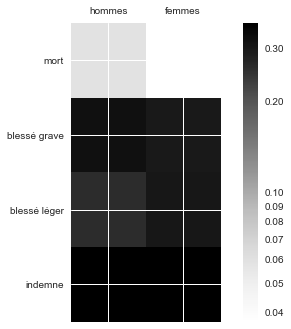
\includegraphics[width=8cm]{colorbar_sex_accident.png}\label{test_sex_accident}
\captionof{figure}{graphical representation of the impact of the sex driver on the accident}

We then run for various independene tests as follows
\begin{verbatim}
Test du chi2 : le sexe du conducteur est-il indépendant 
de la gravité de l’accident ?
La p-value est de 2.19e-31.

Test du chi2 : meurt-on davantage au volant si on est
 une femme ?
La p-value est de 3.55e-18.
La corrélation est de -4.05e-02.

Test du chi2 : est-on davantage mort ou blessé grave
 si on est une femme ?
La p-value est de 1.04e-17.
La corrélation est de -3.99e-02.
\end{verbatim}


\captionof{table}{Impact of driver age on the accident }

\begin{verbatim}
Test du chi2 : l’âge du conducteur est-il indépendant
 de la gravité de l’accident ?
La p-value est de 4.94e-129.

Test du chi2 : meurt-on davantage au volant si on est
 jeune ?
La p-value est de 1.00e+00.
La corrélation est de -3.10e-03.

Test du chi2 : meurt-on **moins** au volant si on est 
jeune ?
La p-value est de 1.00e+00.
La corrélation est de -3.10e-03.

Test du chi2 : est-on davantage mort ou blessé grave
 si on est un jeune ?
La p-value est de 3.39e-35.
La corrélation est de 5.74e-02.


Test du chi2 : meurt-on davantage au volant si on est 
vieux ?
La p-value est de 3.65e-38.
La corrélation est de 5.98e-02.

Test du chi2 : est-on davantage mort ou blessé grave
 si on est un vieux ?
La p-value est de 9.75e-20.
La corrélation est de 4.23e-02.
\end{verbatim}


\begin{verbatim}
Test du chi2 : la bidirectionnalité est-elle indépendante 
de la gravité de l’accident ?
La p-value est de 5.52e-168.

Test du chi2 : indépendance des chances de mourir et 
d’être sur route bidirectionnelle ?
La p-value est de 1.00e+00.
La corrélation est de nan.

Test du chi2 : indépendance des chances de mourir ou
 être blessé grave et d’être sur route bidirectionnelle ?
La p-value est de 8.85e-156.
La corrélation est de -1.14e-01.
\end{verbatim}

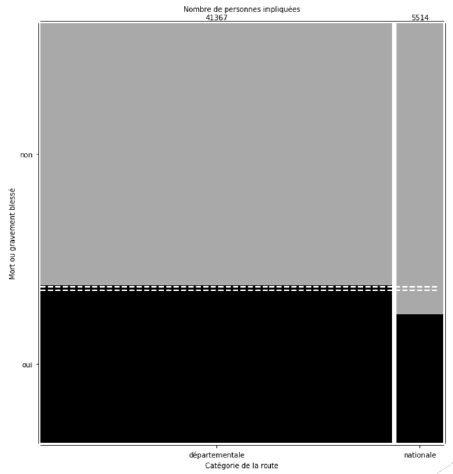
\includegraphics[width=8cm]{indep_1_test2.png}\label{indep_1_test2}
\captionof{figure}{graphical representation of the impact of the type of roads on the accident}

%------------------------------------------------

\end{document}
